


\documentclass[10pt,usletter]{article}
\usepackage[totalwidth=450pt,totalheight=640pt]{geometry}
\date{}
\usepackage{amsthm}


\usepackage{url}\urlstyle{rm}

\usepackage{graphicx,color}

\usepackage{booktabs}
\usepackage{amsmath}
\usepackage{bm}
\usepackage{tikz}



\newenvironment{myquote}{\begin{center}
    \begin{minipage}{.80\linewidth}}{\end{minipage}\end{center}}



\DeclareRobustCommand{\exqed}{\ifmmode
    \eqno \def\@badmath{-3pt]
\small  The University of Texas at Austin, USA
  \and Stefan Szeider\thanks{Research supported by the ERC, grant
    reference 239962 (COMPLEX REASON).}\\
\small  Institute of Information Systems\ \eta_{2,3}( \rho_{2\rightarrow 1}(
    \eta_{2,3}( \eta_{1,2}(1(a) \oplus 2(b)) \oplus 3(c) ) ) \oplus
    2(d) ).
0.1cm]
  \phantom{x}\hfill for , , , .
\end{myquote}

\noindent Together with Lemma~\ref{lem:der} this construction directly yields
the following statement.
\begin{proposition}
  Let  be graph and . Then  
   is satisfiable if and only if . 
\end{proposition}


\begin{example}\label{example:unitprop}
  Let  and . Vertices  in template ,  are in one component, but in different groups.
  Hence the corresponding component variables are true,
  and the corresponding group variables are false.
  The clauses containing the variables 
  with  after removing falsified literals
  are: 
\begin{myquote}
 \\

\end{myquote}
These clauses cannot be satisfied, yet unit propagation will not result in a conflict. 
Therefore, a SAT solver may not be able to cut off the current branch.
\end{example}
 


\subsection{The Representative Encoding}

To overcome the unit propagation problem of the direct encoding, as
described in Example~\ref{example:unitprop}, we propose the {\em
  representative encoding} which uses two types of variables. First,
for each  and  we introduce a representative
variable . This variable, if assigned to true, expresses that
vertex  is the representative of a group in
template~.  In each group, only one vertex can be the
representative and we choose to make the first vertex in the
lexicographical ordering the representative. 
This results in the following clauses:
\begin{myquote}

\qquad for , 


\end{myquote}
\medskip\noindent Additionally we introduce auxiliary variables
to efficiently encode that the number of representative vertices in a
component is at most .
These auxiliary variables are based on the {\em
  order encoding}~\cite{TamuraTagaKitagawaBanbara09}.  Consider a
(non-Boolean) variable  with domain ,
whose elements denote the group number of vertex  in template
. In the direct encoding, we used  variables  with
. Assigning  in that encoding means
.  Alternatively, we can use {\em order variables}
 with , , .  Assigning  means . Consequently,  means .

\begin{examplenoqed} 
Given an assignment to the order variables , one can easily construct the equivalent assignment to the variables in the 
direct encoding (and the other way around). Below is a visualization of the equivalence relation with . In the middle is a binary 
representation of each of the  labels by concatenating the Boolean values to the order variables.
\begin{myquote}
\exqed
\end{myquote}
\end{examplenoqed}

\medskip

Although our encoding is based on the variables from the order encoding, 
we use none of the associated clauses. We implemented the original 
order~\cite{TamuraTagaKitagawaBanbara09}, which resulted 
in many long clauses and the performance was comparable to the direct
encoding.

Instead, we combined the representative and order variables.  Our use
of the order variables can be seen as the encoding of a sequential
counter~\cite{Sinz05}.  We would like to point out that if  and 
are both representative vertices in the same component of template
 and , then  and  must hold for some .  Consequently,
 (vertex  has not the highest group number
in ), \mbox{} (vertex  has not the
lowest group number in ), and \mbox{}:
These constraints can be expressed by the following clauses.
\begin{myquote}
  \quad for , , .
\end{myquote}





\begin{example}
  Consider a graph  with  and the representative encoding with .
  We will show that if ,,, and  are all
  in the same component and they are all
  representatives of their respective group numbers in template , 
  then unit propagation will result in a conflict (because there are four
  representatives and only three group numbers).  Observe that 
   all corresponding component and representative variables are true. 
  This example, with falsified literals removed, contains the clauses
    , 
    , 
    , , 
    , 
    , 
    , 
    , 
    , 
    , 
    \mbox{}, 
    , 
    , 
    , 
    , 
    , 
    , 
    .
Literals that are falsified by unit clauses are shown in bold. 
Notice that  is falsified, i.e., a conflicting clause.
\end{example}

Both the direct and representative encoding require  variables.  The number of clauses depends on the set of edges. In
worst case, the number of clauses can be  due
to the path condition.  





\section{Experimental Results}

In this section we report the results we obtained by running our SAT
encoding on various classes of graphs.  Given a graph , we
compute that  has clique-width  by determining for which value
of  it holds that  is satisfiable and  is unsatisfiable.
We used the SAT solver {\tt Glucose} version 2.2~\cite{Glucose}  to solve the encoded problems. 
{\tt Glucose} solved the hardest instances about twice as fast (or more) as 
other state-of-the-art solvers such as {\tt Lingeling}~\cite{Biere12}, {\tt Minisat}~\cite{Minisat} and {\tt Clasp}~\cite{Clasp}.
We used a 4-core Intel Xeon CPU E31280 3.50GHz,
32 Gb RAM machine running Ubuntu 10.04.


Although the direct and representative encodings result
in CNF formulas of almost equal size, there is a huge difference in
 costs to solve these instances. To determine the
clique-width of the famous named graphs (see below)
using the direct encoding takes about two to three orders of magnitude
longer as compared to the representative encoding.  For example, we can
establish that the Paley graph with 13 vertices has clique-width 9
within a few seconds using the representative encoding, while the
solver requires over an hour using the direct encoding. Because of the
huge difference in speed, we discarded the use of the direct encoding
in the remainder of this section.


We noticed that upper bounds (satisfiable formulas) are obtained
much faster than lower bounds (unsatisfiable formulas). The
reason is twofold.  First,  the whole search space
needs to be explored for lower bounds, while for upper bounds, one can be ``lucky"
and find a solution fast. Second, due to our encoding, upper bound
formulas are smaller (due to a smaller ) which makes them
easier. Table~\ref{tab:random20} shows this for a random graph with 20
vertices for the direct encoding and the representative
encoding. 

\begin{table}[htb]
\centering
\caption{Runtimes in seconds of the direct and representative encoding on a random graph
  with 20 vertices and 95 edges for different values of . Up to  the formulas
  are unsatisfiable, afterwards they are satisfiable. Timeout (TO) is 20,000 seconds.}
\label{tab:random20}

\medskip\small\setlength{\tabcolsep}{4pt}
\begin{tabular}{@{}l@{~~}|@{~~}ccccccc@{~~}|@{~~}ccccccc@{}}
\toprule
~~~ & 3 & 4 & 5 & 6 & 7 & 8 & 9 & 10 & 11 & 12 & 13 & 14 & 15 & 16\\
\midrule
direct & 1.39 & 14.25 & 101.1 & 638.5 & 18,337 & TO & TO & TO & TO & 30.57 & 0.67 & 0.50 & 0.10 & 0.10\\
repres &  0.62 & 2.12 & 8.14 & 12.14 & 33.94 & 102.3 & 358.6 &9.21 & 0.40 & 0.35 &0.32 & 0.29 & 0.29 & 0.28\\
\toprule
\end{tabular}
\end{table}

We examined whether adding symmetry-breaking predicates could improve
performance. We used {\tt Saucy} version 3 for this
purpose~\cite{KatebiSakallahMarkov12}. After the addition of the
clauses with representative variables, the number of symmetries is drastically reduced.
However, one can generate symmetry-breaking
predicates for  and add those instead. Although it is helpful
in some cases, the average speed-up was between 5 to 10\%.

Our experimental computations are ongoing. Below we report on some
of the results we have obtained so far.

\subsection{Random Graphs}


The asymptotics of the clique-width of random graphs have been studied
by Lee et al.~\cite{LeeLeeOum12}.  Their results show that for random
graphs on  vertices the following holds asymptotically almost surely: If the
graphs are very sparse, with an edge probability below , then
clique-width is at most 5; if the edge probability is larger than
, then the clique-width grows at least linearly in .  Our first group
of experiments complements these asymptotic results and provides a
detailed picture on the clique-width of small random graphs.  We have
used the SAT encoding to compute the clique-width of graphs with 10,
15, and 20 vertices, with the edge probability ranging from 0 to~1. A
plot of the distribution is displayed in Figure~\ref{fig:random}.  It is
interesting to observe the symmetry at edge probability , and the
how the steepness of the curve increases with the number of
vertices. Note the ``shoulders'' of the curve for very sparse and very
dense graphs.
\begin{figure}[htb]
\centering
\includegraphics[width=11cm]{random1.pdf}
\caption{Average clique-width of random graphs with edge probabilities between 0
  and~1. Each dot in the graph represents the average
  clique-width of 100 graphs. 
\label{fig:random}}
\end{figure}
  
\subsection{The Clique-Width Numbers}
 
For every , let  denote the smallest number such that there
exists a graph with  vertices that has clique-width~. We call
 the th \emph{clique-width number}.  From the
characterizations known for graphs of clique-width 1, 2, and 3,
respectively~\cite{CornelEtal12}, it is easy to determine the first
three clique-width numbers (, , and ). However, determining
 is not straightforward, as it requires nontrivial arguments to
establish clique-width lower bounds.  We would like to point out that
a similar sequence for the graph invariant \emph{treewidth} is easy to
determine, as the complete graph on  vertices is the smallest graph
of treewidth .  One of the very few known graph classes of
unbounded clique-width for which the exact clique-width can be
determined in polynomial time are
grids~\cite{HeggernesMeisterRotics11}; the  grid with  has clique-width ~\cite{GolumbicRotics00}.  Hence grids
provide the upper bounds , , ,
and .  With our experiments we could determine ,
, , , , and .  It
is known that the path on four vertices () is the unique smallest
graph in terms of the number of vertices with clique-width 3. We could
determine that the triangular prism (\mbox{3-Prism}) is the unique
smallest graph with clique-width , and that there are exactly 7
smallest graphs with clique-width .
There are 68 smallest graphs with clique-width 6 and one of them has
only 18 edges. See Figure~\ref{fig:smallest} for an illustration. 
Additionally, we found several graphs of size 11 with clique-width 7
by extending a graph of size 10 with clique-width 6.



\begin{figure}[ht]
  \centering
  \tikzstyle{every node}=[circle,draw,inner sep=1.5pt,fill=gray]
    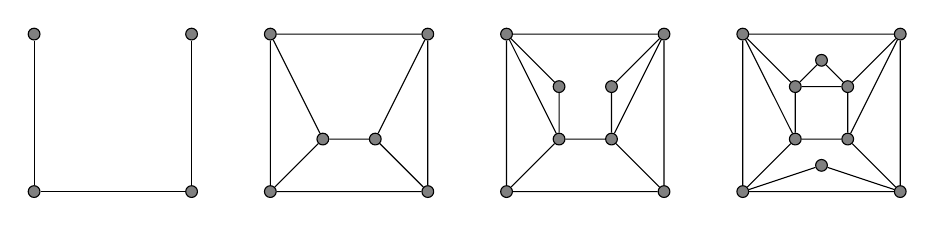
\begin{tikzpicture}
      \draw 
      (0,0)      node (a) {}
      (0,2)      node (b) {}
      (2,0)      node (c) {}
      (2,2)      node (d) {}
      (b)--(a)--(c)--(d)
      ;
    \begin{scope}[xshift=3cm]
      \draw 
      (0,0)      node (a) {}
      (0,2)      node (b) {}
      (2,0)      node (c) {}
      (2,2)      node (d) {}
      (0.667,0.667)    node (e) {}
      (1.333,0.667)    node (g) {}

      (a)--(b)--(d)--(c)--(a)
      (a)--(e)--(b)
      (c)--(g)--(d)
      (e)--(g)
      ;
    \end{scope}
    
        \begin{scope}[xshift=6cm]
      \draw 
      (0,0)      node (a) {}
      (0,2)      node (b) {}
      (2,0)      node (c) {}
      (2,2)      node (d) {}
      (0.667,0.667)    node (e) {}
      (0.667,1.333)    node (f) {}
      (1.333,0.667)    node (g) {}
      (1.333,1.333)    node (h) {}
      (a)--(b)--(d)--(c)--(a)
      (f)--(e)--(g)--(h)
     (a)--(e)
     (b)--(e)
     (b)--(f)
     (c)--(g)
     (d)--(h)
     (d)--(g)
      ;
    \end{scope}
    
        \begin{scope}[xshift=9cm]
      \draw 
      (0,0)      node (a) {}
      (0,2)      node (b) {}
      (2,0)      node (c) {}
      (2,2)      node (d) {}
      (0.667,0.667)    node (e) {}
      (0.667,1.333)    node (f) {}
      (1.333,0.667)    node (g) {}
      (1.333,1.333)    node (h) {}
      (1,0.333)    node (i) {}
      (1,1.667)    node (j) {}
      (a)--(b)--(d)--(c)--(a)
      (e)--(f)--(h)--(g)--(e)
     (a)--(e)
     (b)--(e)
     (b)--(f)
     (c)--(g)
     (d)--(h)
     (d)--(g)
      (a)--(i)--(c)
      (f)--(j)--(h)
      ;
    \end{scope}
\end{tikzpicture}
\caption{Smallest graphs with clique-width 3, 4, 5, and 6 (from left to right).}
  \label{fig:smallest}

\end{figure}


\begin{proposition}
  The clique-width sequence starts with the numbers , , ,
  , , , .
\end{proposition}
We used Brendan McKay's software package Nauty \cite{Mackay81} to
avoid checking isomorphic copies of the same graph.  There are several
other preprocessing methods that can speed up the search for small
graphs of prescribed clique-width .  Obviously, we can limit
the search to \emph{connected} graphs, as the clique-width of a graph
is clearly the maximum clique-width of its connected components. We
can also ignore graphs that contain \emph{twins}---two vertices
that have exactly the same neighbors---as we can delete one of them
without changing the clique-width. Similarly, we can ignore graphs
with a \emph{universal vertex}, a vertex that is adjacent to all other
vertices, as it can be deleted without changing the clique-width. All
these filtering steps are subsumed by the general concept of
\emph{prime graphs}.  Consider a graph . A vertex 
\emph{distinguishes} vertices  if  and . A set  is a \emph{module} if no vertex from
 distinguishes two vertices from . A module  is
\emph{trivial} if . A graph is
\emph{prime} if it contains only trivial modules. It is well-known
that the clique-width of a graph is either  or the maximum
clique-width of its induced prime
subgraphs~\cite{CourcelleOlariu00}. Hence, in our search, we can
ignore all graphs that are not prime. We can efficiently check whether a graph 
is prime~\cite{HabibPaul10}. The larger the number of
vertices, the larger the fraction of non-prime graphs (considering
connected graphs modulo isomorphism).  Table~\ref{table:sequence}
gives detailed results.



 

\begin{table}[htb]
\caption{Number of connected and prime graphs with specified clique-width, modulo isomorphism.}\label{table:sequence}
\centering
\medskip
\begin{tabular}{@{}c@{~~~~~~~~}r@{~~~}r@{~~~~~~}@{~~~}r@{~~~}r@{~~~}r@{~~~}r@{~~~}r@{}}
\toprule
&&& \multicolumn{5}{c}{clique-width}\\
\cmidrule{4-8}
 & connected & prime~ &  &  &  &  & ~~ \\ 
\midrule
4 &             6 &        1   &  0   &          1   &              0   &       0  & 0\\
5 &           21 &       4   &  0   &          4   &              0   &       0  & 0\\
6 &        112 &      26  & 0   &        25   &              1  &        0 & 0\\
7 &        853 &    260  &  0   &      210  &            50   &       0 & 0\\
8 &   11,117 & 4,670  &  0  &     1,873  &      2,790  &        7 & 0\\
9 &   261,080  & 145,870  & 0&  16,348 &   125,364  & 4,158 & 0\\
10 &   11,716,571  & 8,110,354  & 0&  142,745 &   5,520,350  & 2,447,190 & 68\\

\toprule
\end{tabular}
\end{table} 


\subsection{Famous Named Graphs}
\label{sec:famous}

The graph theoretic literature contains several graphs that have
names, sometimes inspired by the graph's topology, and sometimes after
their discoverer. 
We have computed the clique-width of several named graphs,
the results are given in Table~\ref{table:named} (definitions of all
considered graphs can be found in MathWorld \cite{MathWorld}).  The
\emph{Paley graphs}, named after the English mathematician Raymond
Paley (1907--1933), stick out as having large clique-width. Our
results on the clique-width of Paley graphs imply some upper bounds on
the 9th and 11th clique-width numbers:  and .
 
\begin{table}[htb]
\centering
\caption{Clique-width of named graphs. Sizes are reported for the unsatisfiables.}\label{table:named}
\medskip
\begin{tabular}{l@{\hspace{5mm}}r@{\hspace{5mm}}r@{\hspace{5mm}}r@{\hspace{5mm}}r@{\hspace{5mm}}r@{\hspace{5mm}}r@{\hspace{5mm}}r}
\toprule
graph &  & & cwd & variables & clauses & UNSAT  & SAT \\ 
\midrule
Brinkmann & 21 & 42 & 10 & 8,526 & 163,065 & 3,932.56 & 1.79\\Chv\'{a}tal   &                12 & 24 & 5 & 1,800 & 21,510 & 0.40 & 0.09 \\Clebsch &                 16 & 40 & 8 & 3,872 & 60,520 & 191.02 & 0.09\\Desargues &             20 & 30 & 8 & 7,800 & 141,410 & 3,163.70 & 0.26\\Dodecahedron &      20 & 30 & 8 & 7,800 & 141,410 & 5,310.07 & 0.33\\Errera     &                17 & 45 & 8 & 4,692  & 79,311 & 82.17 & 0.16\\Flower snark &      20 & 30 & 7 & 8,000 & 148,620 & 276.24 & 3.9\\Folkman &                20 & 40 & 5 & 8,280 & 168,190 & 11.67 & 0.36\\Franklin &               12 & 18 & 4 & 1,848 & 21,798 & 0.07 & 0.04\\Frucht   &               12 & 18 & 5 & 1,800 & 20,223 & 0.39 & 0.02\\Hoffman &           16  & 32 & 6 & 4,160 & 64,968 & 8.95 & 0.46\\Kittell  &                23  & 63 & 8 & 12,006 & 281,310 & 179.62 & 18.65\\McGee &              24  & 36 & 8 & 13,680 &  303,660 & 8,700.94 & 59.89\\Sousselier &       16  & 27 & 6 & 4,160  & 63,564 & 3.67 & 11.75\\Paley-13  &         13 & 39 & 9 & 1,820 & 22,776 & 12.73 & 0.05 \\ Paley-17 &         17 & 68 & 11 & 3,978 & 72,896 & 194.38 & 0.12\\ Pappus  &            18 & 27 & 8 & 5,616 & 90,315 & 983.67 & 0.14\\Petersen   &         10 & 15 & 5 & 1,040 & 9,550 & 0.10 & 0.02\\ Poussin &            15 & 39 & 7 & 3,300 & 50,145 & 9.00 & 0.21\\Robertson &        19 & 38 & 9 & 6,422 & 112, 461 & 478.83 & 0.76\\ Shrikhande &       16 & 48 & 9 & 3,680 & 59,688 & 129.75 & 0.11\\\toprule
\end{tabular}
\end{table}


\section{Conclusion}

We have presented a SAT approach to the exact computation of
clique-width, based on a reformulation of clique-width and several
techniques to speed up the search.  This new approach allowed us to
systematically compute the exact clique-width of various small graphs.  
We think that our results could be of relevance for theoretical investigations. 
For instance, knowing small vertex-minimal graphs of certain clique-width 
could be helpful for the design
of discrete algorithms that recognize graphs of bounded
clique-width. Such graphs can also be useful as gadgets for a
reduction to show that the recognition of graphs of clique-width~4 is
\hy hard, which is still a long-standing open problem
\cite{FellowsRosamondRoticsSzeider09}.  Furthermore, as discussed in
Section~\ref{sect:intro}, there are no heuristic algorithms to compute
the clique-width directly, but heuristic algorithms for related
parameters can be used to obtain upper bounds on the clique-width. Our
SAT-based approach can be used to empirically evaluate how far
heuristics are from the optimum, at least for small and
medium-sized graphs. 

So far we have focused in our experiments on the exact clique-width,
but for various applications it is sufficient to have  good upper
bounds. Our results (see Table~\ref{tab:random20}) suggest that our
approach can be scaled to medium-sized graphs for the computation of
upper bounds.  We also observed that for many graphs the upper bound
of Lemma~\ref{lem:strict-shorter} is not tight. Thus, we expect that
if we search for shorter derivations, which is significantly faster,
this will yield optimal or close to optimal solutions in many cases.


Finally, we would like to mention that our SAT-based approach is very
flexible and open. It can easily be adapted to variants of
clique-width, such as linear clique-width
\cite{HeggernesMeisterPapadopoulos12,FellowsRosamondRoticsSzeider09},
\hy clique-width \cite{CourcelleTwigg10}, or
NLC-width~\cite{Wanke94}. Hence, our approach can be used for an
empirical comparison of these parameters.

\section*{Acknowledgement}
The authors acknowledge the Texas Advanced Computing Center (TACC) at The University of Texas at 
Austin for providing grid resources that have contributed to the research results reported within this paper.

\begin{thebibliography}{10}

\bibitem{Glucose}
Gilles Audemard and Laurent Simon.
\newblock Predicting learnt clauses quality in modern sat solvers.
\newblock In {\em Proceedings of the 21st international jont conference on
  Artifical intelligence}, IJCAI'09, pages 399--404, San Francisco, CA, USA,
  2009. Morgan Kaufmann Publishers Inc.

\bibitem{Beyss2013}
Martin Bey\ss.
\newblock Fast algorithm for rank-width.
\newblock In {\em Mathematical and Engineering Methods in Computer Science, 8th
  International Doctoral Workshop, MEMICS 2012, Znojmo, Czech Republic, October
  25-28, 2012, Revised Selected Papers}, volume 7721 of {\em Lecture Notes in
  Computer Science}, pages 82--93. Springer Verlag, 2013.

\bibitem{Biere12}
Armin Biere.
\newblock Lingeling and friends entering the {SAT} {Challenge} 2012.
\newblock In A.~Balint, A.~Belov, A.~Diepold, S.~Gerber, M.~J\"{a}rvisalo, and
  C.~Sinz, editors, {\em Solver and Benchmark Descriptions}, volume B-2012-2 of
  {\em Department of Computer Science Series of Publications B.}, pages 33--34.
  University of Helsinki, 2012.

\bibitem{BuixuanTelleVatshelle11}
Binh-Minh Bui-Xuan, Jan~Arne Telle, and Martin Vatshelle.
\newblock Boolean-width of graphs.
\newblock {\em Theoretical Computer Science}, 412(39):5187--5204, 2011.

\bibitem{CornelEtal12}
Derek~G. Corneil, Michel Habib, Jean-Marc Lanlignel, Bruce Reed, and Udi
  Rotics.
\newblock Polynomial-time recognition of clique-width {} graphs.
\newblock {\em Discr. Appl. Math.}, 160(6):834--865, 2012.

\bibitem{CornelRotics05}
Derek~G. Corneil and Udi Rotics.
\newblock On the relationship between clique-width and treewidth.
\newblock {\em SIAM J. Comput.}, 34(4):825--847, 2005.

\bibitem{CourcelleMakowskyRotics00}
B.~Courcelle, J.~A. Makowsky, and U.~Rotics.
\newblock Linear time solvable optimization problems on graphs of bounded
  clique-width.
\newblock {\em Theory Comput. Syst.}, 33(2):125--150, 2000.

\bibitem{CourcelleMakowskyRotics01}
B.~Courcelle, J.~A. Makowsky, and U.~Rotics.
\newblock On the fixed parameter complexity of graph enumeration problems
  definable in monadic second-order logic.
\newblock {\em Discr. Appl. Math.}, 108(1-2):23--52, 2001.

\bibitem{CourcelleOlariu00}
B.~Courcelle and S.~Olariu.
\newblock Upper bounds to the clique-width of graphs.
\newblock {\em Discr. Appl. Math.}, 101(1-3):77--114, 2000.

\bibitem{CourcelleEngelfrietRozenberg90}
Bruno Courcelle, Joost Engelfriet, and Grzegorz Rozenberg.
\newblock Context-free handle-rewriting hypergraph grammars.
\newblock In Hartmut Ehrig, Hans-J{\"o}rg Kreowski, and Grzegorz Rozenberg,
  editors, {\em Graph-Grammars and their Application to Computer Science, 4th
  International Workshop, Bremen, Germany, March 5--9, 1990, Proceedings},
  volume 532 of {\em Lecture Notes in Computer Science}, pages 253--268, 1991.

\bibitem{CourcelleEngelfrietRozenberg93}
Bruno Courcelle, Joost Engelfriet, and Grzegorz Rozenberg.
\newblock Handle-rewriting hypergraph grammars.
\newblock {\em J. of Computer and System Sciences}, 46(2):218--270, 1993.

\bibitem{CourcelleTwigg10}
Bruno Courcelle and Andrew Twigg.
\newblock Constrained-path labellings on graphs of bounded clique-width.
\newblock {\em Theory Comput. Syst.}, 47(2):531--567, 2010.

\bibitem{Diestel00}
Reinhard Diestel.
\newblock {\em Graph Theory}, volume 173 of {\em Graduate Texts in
  Mathematics}.
\newblock Springer Verlag, New York, 2nd edition, 2000.

\bibitem{DowKorf07}
P.~Alex Dow and Richard~E. Korf.
\newblock Best-first search for treewidth.
\newblock In {\em Proceedings of the Twenty-Second AAAI Conference on
  Artificial Intelligence, July 22-26, 2007, Vancouver, British Columbia,
  Canada}, pages 1146--1151. AAAI Press, 2007.

\bibitem{Minisat}
Niklas E\'en and Niklas S\"orensson.
\newblock An extensible sat-solver.
\newblock In Enrico Giunchiglia and Armando Tacchella, editors, {\em Theory and
  Applications of Satisfiability Testing}, volume 2919 of {\em Lecture Notes in
  Computer Science}, pages 502--518. Springer Berlin Heidelberg, 2004.

\bibitem{FellowsRosamondRoticsSzeider09}
Michael~R. Fellows, Frances~A. Rosamond, Udi Rotics, and Stefan Szeider.
\newblock Clique-width is {NP}-complete.
\newblock {\em SIAM J. Discrete Math.}, 23(2):909--939, 2009.

\bibitem{Clasp}
M.~Gebser, B.~Kaufmann, A.~Neumann, and T.~Schaub.
\newblock clasp: A conflict-driven answer set solver.
\newblock In C.~Baral, G.~Brewka, and J.~Schlipf, editors, {\em Proceedings of
  the Ninth International Conference on Logic Programming and Nonmonotonic
  Reasoning (LPNMR'07)}, volume 4483 of {\em Lecture Notes in Artificial
  Intelligence}, pages 260--265. Springer-Verlag, 2007.

\bibitem{Gent02}
Ian~P. Gent.
\newblock Arc consistency in {SAT}.
\newblock In F.~{van Harmelen}, editor, {\em 15th European Conference on
  Artificial Intelligence (ECAI 2002)}, pages 121--125. IOS Press, 2002.

\bibitem{GogateDechter04}
Vibhav Gogate and Rina Dechter.
\newblock A complete anytime algorithm for treewidth.
\newblock In {\em Proceedings of the Proceedings of the Twentieth Conference
  Annual Conference on Uncertainty in Artificial Intelligence (UAI-04)}, pages
  201--208, Arlington, Virginia, 2004. AUAI Press.

\bibitem{GolumbicRotics00}
Martin~Charles Golumbic and Udi Rotics.
\newblock On the clique-width of some perfect graph classes.
\newblock {\em Internat. J. Found. Comput. Sci.}, 11(3):423--443, 2000.
\newblock Selected papers from the Workshop on Graph-Theoretical Aspects of
  Computer Science (WG 99), Part 1 (Ascona).

\bibitem{HabibPaul10}
Michel Habib and Christophe Paul.
\newblock A survey of the algorithmic aspects of modular decomposition.
\newblock {\em Computer Science Review}, 4(1):41--59, 2010.

\bibitem{HeggernesMeisterPapadopoulos12}
Pinar Heggernes, Daniel Meister, and Charis Papadopoulos.
\newblock Characterising the linear clique-width of a class of graphs by
  forbidden induced subgraphs.
\newblock {\em Discr. Appl. Math.}, 160(6):888--901, 2012.

\bibitem{HeggernesMeisterRotics11}
Pinar Heggernes, Daniel Meister, and Udi Rotics.
\newblock Computing the clique-width of large path powers in linear time via a
  new characterisation of clique-width.
\newblock In Alexander~S. Kulikov and Nikolay~K. Vereshchagin, editors, {\em
  Computer Science - Theory and Applications - 6th International Computer
  Science Symposium in Russia, CSR 2011, St. Petersburg, Russia, June 14-18,
  2011. Proceedings}, volume 6651 of {\em Lecture Notes in Computer Science},
  pages 233--246. Springer Verlag, 2011.

\bibitem{HvidevoldEtal11}
Eivind~Magnus Hvidevold, Sadia Sharmin, Jan~Arne Telle, and Martin Vatshelle.
\newblock Finding good decompositions for dynamic programming on dense graphs.
\newblock In D{\'a}niel Marx and Peter Rossmanith, editors, {\em Parameterized
  and Exact Computation - 6th International Symposium, IPEC 2011,
  Saarbr{\"u}cken, Germany, September 6-8, 2011. Revised Selected Papers},
  volume 7112 of {\em Lecture Notes in Computer Science}, pages 219--231.
  Springer Verlag, 2012.

\bibitem{KatebiSakallahMarkov12}
Hadi Katebi, Karem~A. Sakallah, and Igor~L. Markov.
\newblock Conflict anticipation in the search for graph automorphisms.
\newblock In Nikolaj Bj{\o}rner and Andrei Voronkov, editors, {\em Logic for
  Programming, Artificial Intelligence, and Reasoning - 18th International
  Conference, LPAR-18, M{\'e}rida, Venezuela, March 11-15, 2012. Proceedings},
  volume 7180 of {\em Lecture Notes in Computer Science}, pages 243--257.
  Springer Verlag, 2012.

\bibitem{KosterBodlaenderHoesel01}
Arie M. C.~A. Koster, Hans~L. Bodlaender, and Stan P.~M. van Hoesel.
\newblock Treewidth: Computational experiments.
\newblock {\em Electronic Notes in Discrete Mathematics}, 8:54--57, 2001.

\bibitem{LeeLeeOum12}
Choongbum Lee, Joonkyung Lee, and Sang-il Oum.
\newblock Rank-width of random graphs.
\newblock {\em J. Graph Theory}, 70(3):339--347, 2012.

\bibitem{Mackay81}
Brendan~D. McKay.
\newblock Practical graph isomorphism.
\newblock In {\em Proceedings of the {T}enth {M}anitoba {C}onference on
  {N}umerical {M}athematics and {C}omputing, {V}ol. {I} ({W}innipeg, {M}an.,
  1980)}, volume~30, pages 45--87, 1981.

\bibitem{Oum08}
{Sang-il} Oum.
\newblock Approximating rank-width and clique-width quickly.
\newblock {\em ACM Transactions on Algorithms}, 5(1), 2008.

\bibitem{OumSeymour06}
{Sang-il} Oum and P.~Seymour.
\newblock Approximating clique-width and branch-width.
\newblock {\em J. Combin. Theory Ser. B}, 96(4):514--528, 2006.

\bibitem{SamerVeith09}
Marko Samer and Helmut Veith.
\newblock Encoding treewidth into {SAT}.
\newblock In {\em Theory and Applications of Satisfiability Testing - SAT 2009,
  12th International Conference, SAT 2009, Swansea, UK, June 30 - July 3, 2009.
  Proceedings}, volume 5584 of {\em Lecture Notes in Computer Science}, pages
  45--50. Springer Verlag, 2009.

\bibitem{Sinz05}
Carsten Sinz.
\newblock Towards an optimal cnf encoding of boolean cardinality constraints.
\newblock In Peter van Beek, editor, {\em Principles and Practice of Constraint
  Programming - CP 2005, 11th International Conference, CP 2005, Sitges, Spain,
  October 1-5, 2005, Proceedings}, volume 3709 of {\em Lecture Notes in
  Computer Science}, pages 827--831. Springer Verlag, 2005.

\bibitem{SmithUlusalHicks12}
J.~Cole Smith, Elif Ulusal, and Illya~V. Hicks.
\newblock A combinatorial optimization algorithm for solving the branchwidth
  problem.
\newblock {\em Comput. Optim. Appl.}, 51(3):1211--1229, 2012.

\bibitem{TamuraTagaKitagawaBanbara09}
Naoyuki Tamura, Akiko Taga, Satoshi Kitagawa, and Mutsunori Banbara.
\newblock Compiling finite linear {CSP} into {SAT}.
\newblock {\em Constraints}, 14(2):254--272, 2009.

\bibitem{Walsh00}
Toby Walsh.
\newblock {SAT} v {CSP}.
\newblock In R.~Dechter, editor, {\em 6th International Conferenc on Principles
  and Practice of Constraint Programming (CP 2000)}, volume 1894 of {\em
  Lecture Notes in Computer Science}, pages 441--456. Springer Verlag, 2000.

\bibitem{Wanke94}
Egon Wanke.
\newblock {}-{NLC} graphs and polynomial algorithms.
\newblock {\em Discr. Appl. Math.}, 54(2-3):251--266, 1994.
\newblock Efficient algorithms and partial -trees.

\bibitem{MathWorld}
Eric Weisstein.
\newblock {MathWorld} online maathematics resource.

\end{thebibliography}




\end{document}
